\documentclass{article}
\usepackage{geometry}
\geometry{a4paper}
\usepackage{amsmath}
\usepackage{empheq}
\usepackage{mhchem} % Package for chemical equation typesetting
\usepackage{siunitx} % Provides the \SI{}{} command for typesetting SI units
\usepackage{parskip}
\usepackage{graphicx} % Required for the inclusion of images
\usepackage{amssymb}
\usepackage{placeins}
\usepackage{cancel}
\usepackage{fullpage}
%\usepackage{subfig}
\usepackage{enumitem}
\usepackage{listings}
%\usepackage{mcode}
\usepackage{wrapfig}
%\renewcommand{\labelenumii}{\alph{enumi}.}
%Alph for uppcer case, \arabic for 1, 2, 3
%\roman for i, ii, iii \alph{enumi})
% Make numbering in the enumerate environment by letter rather than number (e.g. section 6)
\usepackage{booktabs, multicol, multirow}
%\usepackage[ ]{mcode} 

\setlength\parindent{0pt} % Removes all indentation from paragraphs

\renewcommand{\labelenumi}{\alph{enumi}.} % Make numbering in the enumerate environment by letter rather than number (e.g. section 6)

%\usepackage{times} % Uncomment to use the Times New Roman font

\include{paulsmacros}
%\braces , \parens \brackets \mC (matrix C) \vv (vector v) \h hats for somethings ie \hvy or \hmA \sA (subscript upper case)
\usepackage{caption}
\usepackage{subcaption}

%----------------------------------------------------------------------------------------
%	DOCUMENT INFORMATION
%----------------------------------------------------------------------------------------
%$\frac{-1}{\sqrt{a}}$
%\title{Newberry/Felix  \hfill \today}
%\date{}
\begin{document}
%\maketitle 
%\LARGE
\textsc{\Large FSIr Validation \hfill \today}\\[0.5cm] % Name of your university/college
\textsc{\large Felix Newberry}\\

This report describes the validation of a Fenics fluids structure interaction (FSI) solver. The fluid and structure sections have been validated separately. This report details the validation of the interaction. 
%The code in question can be found in the Github repository under \verb|/2_Cylinder_benchmark/cylinder_navier-stokes.py|. 

\section{Problem Setup} 

The benchmark problem of 2D flow in a channel pasta  cylinder with an elastic bar attached is solved. The problem is solved with a partitioned  Arbitary Lagrangian-Eulerian (ALE) method. 

The fluid problem is solved with an Incremental Pressure Correction Scheme (IPCS). The fluid solver has been validated with a 2D benchmark channel flow past a circular cylinder \cite{schafer1996benchmark}. 

The nonlinear dynamic structure problem is solved in Fenics with the $CG_1$ method \cite{eriksson1996computational}. The method is described in chapter 27 of the Fenics book that addresses nonlinear elasticity \cite{logg2012automated}. Speicifically, 27.2.3 details time-stepping algorithims for nonlinear elastic models. The structure solver was validated with the structure test case of an elastic beam attatched to a cylinder \cite{turek2006proposal}. 

\subsection{Geometry}
The geometry of the computational domain is depicted in Figure \ref{fig:domain} and the structure detail in Figure \ref{fig:structre} \cite{turek2006proposal}. 

\FloatBarrier
\begin{figure}[h]
\centering
	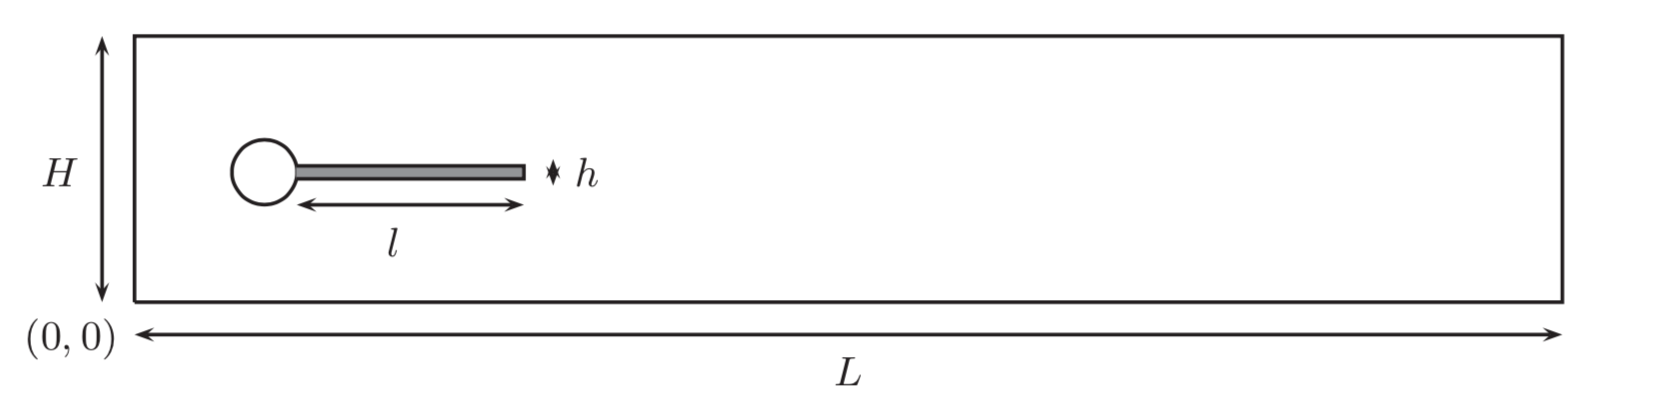
\includegraphics[width=\textwidth]{domain}
	\caption{Computational domain \cite{turek2006proposal}}
	\label{fig:domain}
\end{figure}
\FloatBarrier

\FloatBarrier
\begin{figure}[h]
\centering
	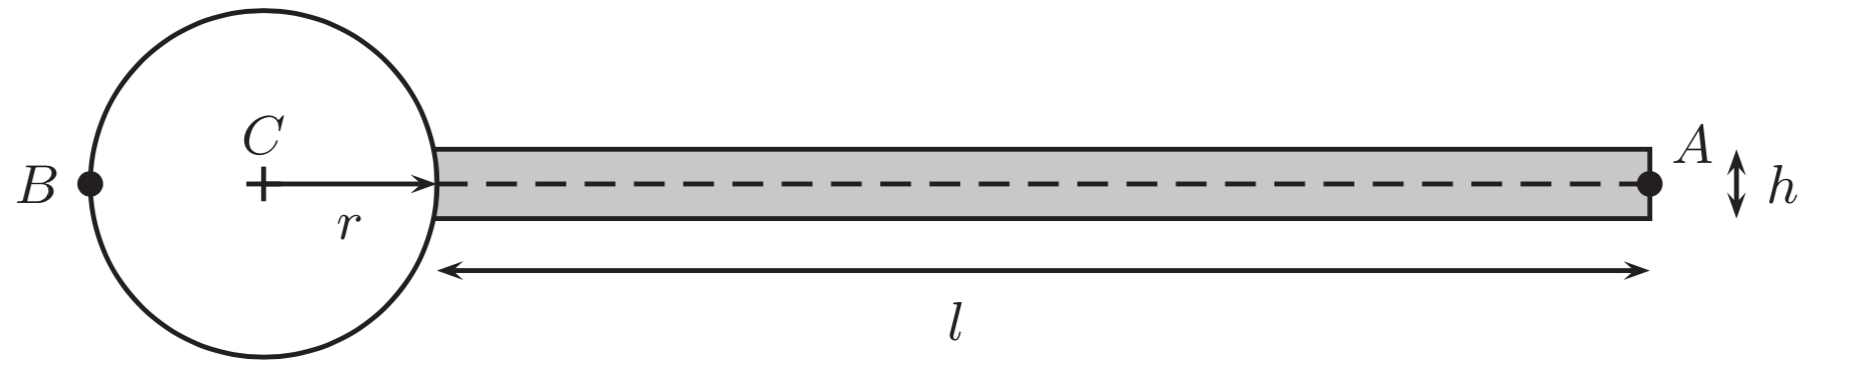
\includegraphics[width=\textwidth]{struct_geom}
	\caption{Structure detail \cite{turek2006proposal}}
	\label{fig:structre}
\end{figure}
\FloatBarrier

A circular cylinder of diameter $D = 0.1 m$ is centered at $h = 0.2 m$ and $0.2 m$ from the inlet in a channel of height $H = 0.41 m$. The channel length is set as $L = 2.5 m$. An elastic bar of length $l = 0.35 m$ and height $h = 0.02 m$ has it's bottom right corner positioned at $(0.6, 0.19)$ and the left end fully attached to the fixed cylinder. Control points are $A(t)$ on the structure with $A(0) = (0.6, 0.2)$, and $B = (0.15, 0.12)$. 

\subsection{Fluid Properties}
The fluid considered is incompressible and Newtonian. The kinematic viscosity was defined as $\nu = 0.001 m^2s^{-1}$ and the density as $ \rho = 1000.0 kg m^{-3}$. 

\subsection{Structure Properties}
The structure is modeled as elastic and compressible. The material is St. Venant-Kirchhoff. The first lame constant was defined as $\mu = 0.05 kg m^{-1}s^{-2}$, the Poisson ratio as $\nu = 0.4$ and the density as $\rho = 1000 kg m^{-3}$.

\subsection{Boundary Conditions}
The channel walls and the surface of the cylinder are no-slip condition while the outlet pressure is set to 0. The inflow is a parabolic velocity profile in the x direction defined as 

\begin{equation}
U(0, y) = \frac{4 U_m y (H - y)}{H^2} , V = 0
\end{equation}

where $U_m = 0.3$ is the maximum velocity of the inlet and the mean velocity is defined as $\bar{U}$. 

The boundary conditions on the fluid structure interface are defined as

\begin{align}
\mathbf{\sigma}_f \cdot \mathbf{n}_f &= -\sigma_s \cdot \mathbf{n}_s\\
 \mathbf{v}_f &= \mathbf{v}_s \\
\end{align}


where the fluid, $f$ or structure, $s$, stress, $\mathbf{\sigma}$ and normal vector, $\mathbf{n}$, ensure the traction forces of each boundary are equal. Likewise the the fluid and structure velocities $\mathbf{v}$ are equal. 

\subsection{FSI Solver}

The FSI problem is divided into three sub-problems comprised of the fluid, structure and mesh. For a given timestep solver sequence can be described as

\begin{itemize}
\item Solve fluid problem 
\item Compute traction applied to structure from fluid and solve structure problem
\item Solve mesh problem with structure interface velocity as boundary condition
\item Repeat steps 1-3 until convergence
\item Move to the subsequent time step
\end{itemize}



The structure is solved in a Lagrangian framework in which the structure mesh moves with the structure. The fluid is solved in an Eulerian framework where motion of the fluid is related to a fixed spatial point $x$. The deformation of the structure has to be tracked in the fluid domain by deforming the fluid mesh. Therefore an additional mesh smoothing algorithm is introduced in order to have the mesh move with the structure. The Lagrangian, Eulerian and mesh smoothing algorithm comprise the Arbitrary Lagrangian-Eulerian (ALE) method. 

To make these two reference domains compatible an arbitrary reference frame is introduced which is independent from both the Lagrangian and Eulerian descriptions. The arbitrary reference frame is set as the undeformed computational domain and denoted as $\Omega$. The reference domain is comprised of the fluid and structure domains such that $\Omega_F \cup \Omega_S = \Omega$ and $\Omega_F \cap \Omega_S = 0$ for $ t \in [0,T]$. 
The current, deformed, computational domain is similarly denoted by $\omega_F \cup \omega_S = \omega$ and $\omega_F \cap \omega_S = 0$ for $ t \in [0,T]$. The common boundary is given by $\Gamma_{FSI}$ and $\gamma_{FSI}(t)$ respectively. As a general rule, upper case variables relate to the reference domain and lower case to the deformed domain. 

To map between the current and reference domains the bijective map $\Phi (\cdot , t) : \Omega \rightarrow \omega(t)$ is introduced. $\Phi$ maps a reference point $X \in \Omega$ to the corresponding current point $x \in \omega(t)$. Thus $X \rightarrow x = \Phi (X,t)$. 




The mesh is solved with a linear elastic description of fluid domain in which the stress tensor is given by 
$\Sigma_M (U_M) = \mu_M (Grad (U_M) + Grad (U_M^T) + \lambda_M tr ( Grad(U_M) I$ for some positive constants $ (\mu_M, \lambda_M$. 

In summation: 

\begin{itemize}
\item the fluid problem is solved in the current fluid domain $\omega_F(t)$
\item the structure problem is solved in the reference structure domain $\Omega_S$
\item the mesh problem is solved in the reference fluid domain $\Omega_F$
\end{itemize}

The mesh equation reads as 

\begin{equation}
\dot{U}_M - Div \: \Sigma_M (U_M) = 0 \hspace{1cm} \text{in } \Omega_F \times (0, T]
\end{equation}

The fluid stress is computed as the cauchy stress tensor
\begin{equation}
\sigma_F = 2 \mu_F \epsilon( u_F) - p_F* I 
\end{equation}

where $\mu_F$ is they dynamic viscosity and $\epsilon$ the symmetric gradient. This stress is communicated to the structure domain as 

\begin{equation}
(J_M (\sigma_F \circ \Phi_M) \cdot F_M^{-T} ) \cdot N_F = -\Sigma_S \cdot N_S  \hspace{1cm} \text{on } \Gamma_{FS}
\end{equation}

where $J$ = $det(F)$ is the determinant of the Jacobi matrix $F = Grad (\phi)$ and $N_F$ and $N_S$ are the respective fluid and structure mesh facet normals. $\phi$ defines the structure displacement comparing to the reference position as $u(X,t) = \\phi(X,t) - X$. 
 
Kinematic continuity is asserted through matching the structure and mesh velocities 
\begin{equation}
u_F \circ \Phi_M = \dot{U}_S
\end{equation}

Evidently the map between the fluid and the mesh is crucial. 

Finally, the fluid solver is adjusted to allow for the non-physical mesh movement in the convective term $\rho_F (\dot{u}_F+ u_F \cdot( u_F-\dot{u}_M))$

Need mesh solution to be based on reference domain: undeformed mesh. The tricky but will be communcating the mesh velocity to the fluid. 

\subsection{Validation Metrics}
The metrics for validation are the drag and lift forces , $F_D$ and $F_L$ on the cylinder and structure boundary as a whole and  the x and y displacement of point A. The drag and lift forces were calculated as 

\begin{equation}
F_D = \int ( \rho \nu \frac{\partial v_t}{\partial n}  n_y - P n_x ) dS
\end{equation}

\begin{equation}
F_L = - \int ( \rho \nu \frac{\partial v_t}{\partial n}  n_x - P n_y ) dS
\end{equation}

where $S$ denotes the entire integration path of the cylinder and structure, $n$ is the normal vector on $S$ with x and y components $n_x$ and $n_y$. $v_t$ is the tangential velocity on $S$ with tangent vector $t = (n_y - n_x)$ and $P$ is the pressure. $S = S_0 +S_1$ where $S_0$ and $S_1$ are the integration paths of the cylinder and structure along their boundaries with the fluid. 

\subsection{Mesh}

The Mesh used in this analysis was constructed in GMSH. A separate mesh was created for both the fluid and structure domains and each one loaded independently into Fenics. It was ensured that the nodes on the fluid structure boundary between the two meshes are coincident. 

A course mesh of the fluid region is depicted in Figure \ref{fig:mesh_fluid} and of the structure in Figure \ref{fig:mesh_structure}. 

\FloatBarrier
\begin{figure}[h]
\centering
	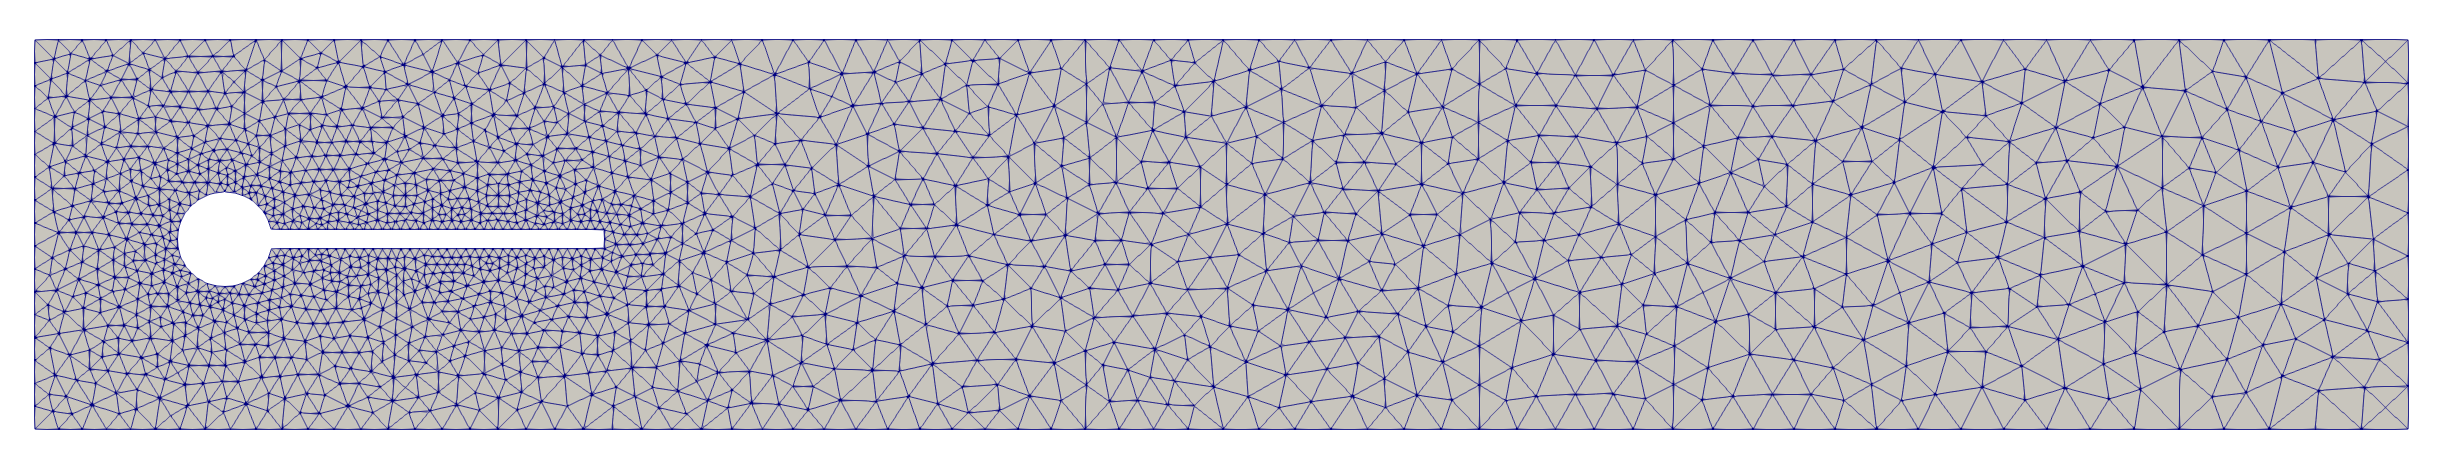
\includegraphics[width=0.6\textwidth]{mesh_fluid}
	\caption{Course mesh of fluid domain}
	\label{fig:mesh_fluid}
\end{figure}
\FloatBarrier

\FloatBarrier
\begin{figure}[h]
\centering
	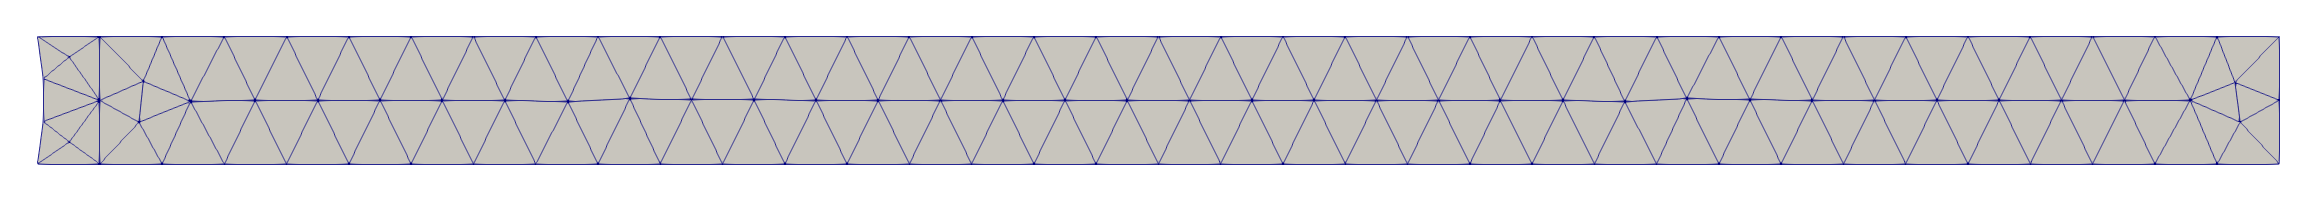
\includegraphics[width=0.6\textwidth]{mesh_structure}
	\caption{Course mesh of structure domain}
	\label{fig:mesh_structure}
\end{figure}
\FloatBarrier

\section{Validation} 

%The mesh refinement results of $C_D$, $C_L$ and $P_{diff}$ are presented in Table \ref{tab:fluid}. Figures \ref{fig:drag}, \ref{fig:lift} and \ref{fig:p_diff} illustrate mesh convergence to the benchmark solution for coefficients of drag and lift, and the pressure difference respectively. The red lines indicate the benchmark solution lower and upper bounds \cite{schafer1996benchmark}.   

%\FloatBarrier
 % \begin{table}[htbp]
  %\setlength\extrarowheight{5pt}
  %\centering
  %\caption{Results of mesh independence study}
   % \begin{tabular}{ccccc}
   % \toprule
    %$N$ & $ndof$ & $C_D$ & $C_L$ & $P_{diff}$ \\
    %\midrule
%$32$ & $8503$ & $5.512$ & $-0.01117$ & $0.1142$ \\
%$64$ & $28760$ & $5.557$ & $0.01018$ & $0.1169$ \\
%$128$ & $108217$ & $5.569$ & $0.01103$ & $0.1173$ \\
%$256$ & $416630$ & $5.574$ & $0.01094$ & $0.1174$ \\
  %  \bottomrule
  %  \end{tabular}%
  %\label{tab:fluid}%
%\end{table}%
%\FloatBarrier

%Figures \ref{fig:drag}, \ref{fig:lift} and  \ref{fig:p_diff} all demonstrate convergence to the benchmark solution. Further mesh refinement is necessary to confirm mesh independence. The majority of the 17 methods presented in the benchmark solution to arrive at the bounds have a much higher grid refinement, 6 of them have an order of magnitude more more dofs. 



\bibliography{validation}{}
\bibliographystyle{plain}


\end{document}
